\documentclass[12pt]{article}
\usepackage{amsmath}
\usepackage[T1]{fontenc}
\usepackage{graphicx}
\usepackage{amsfonts}
\usepackage{tikz}
\usepackage{listings}
\newcommand{\floor}[1]{\left\lfloor #1 \right\rfloor}	% podłoga
\newcommand{\ceil}[1]{\left\lceil #1 \right\rceil}		% sufit
\newcommand{\fractional}[1]{\left\{ #1 \right\}}		% część ułamkowa {x}
\newcommand{\abs}[1]{\left| #1 \right|}					% wartosc bezwzgledna / moc
\newcommand{\set}[1]{\left \{ #1 \right \}}				% zbiór elementów {a,b,c}
\newcommand{\pair}[1]{\left( #1 \right)}				% para elementów (a,b
\title{AISD lista 4}
\author{Dominik Szczepaniak}
\begin{document}

\maketitle

\bgroup\obeylines

\section{Zadanie 3}
Ukorzenimy drzewo w centroidzie i uzyjemy algorytmu z wykladu dla drzew ukorzenionych.

\section{Zadanie 4}


ALGORYTM HOARE'A
\begin{lstlisting}
    def mediana(arr, l, r, k): # mediana to k-ty najmniejszy element

        if (k > 0 and k <= r - l + 1):

            index = partition(arr, l, r)
            
            if (index - l == k - 1):
                return arr[index]
            if (index - l > k - 1):
                return mediana(arr, l, index - 1, k)
            return mediana(arr, index + 1, r, k - index + l - 1)
        return INT_MAX
\end{lstlisting}

Rozpatrzmy rozmiary kolejnych podtablic powstałych w wyniku podziału.
Z artykułu wiemy, że optymistyczny rozmiar kolejnej tablicy to conajwyżej$\frac{3}{4}$ rozmiaru rodzica. Jest to podział zrównoważony.
Analaogicznie podziała wykraczający rozmiarem nowo powstałej tablicy poza $\frac{3}{4}$ rozmiaru rodzica nazywamy podziałem niezrównoważonym. 

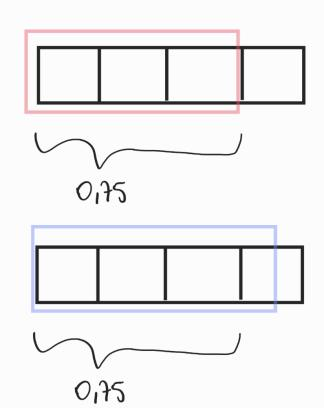
\includegraphics[scale=0.5]{zad4_1.png}

Powstałą tablicy która jest zrównoważona będziemy oznaczać jako czerwone dziecko.
Tablicę, które jest niezrównoważona będziemy nazywać niebieskim dzieckiem.

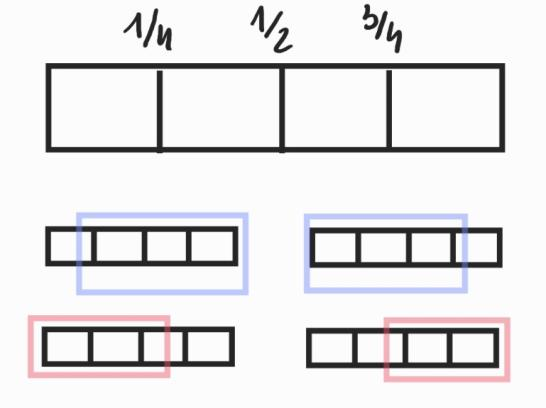
\includegraphics[scale=0.5]{zad4_2.png}

Podział zrównoważony otrzymamy z prawdopodobieństwem co najmniej $\frac{1}{2}$. 
Wynika to z jednostajnego rozkładu prawdopodobieństwa. 

Pivot może zajmować jedną z $n$ pozycji. Jeżeli zwrócimy uwagę na rozmiar powstałej w w wyniku takiego podziału lewej podtablicy, to otrzymamy, że ten podział może mieć długość od $0$ do $n-1$.

Niezrównoważony podział wystąpi, gdy lewy podział będzie mniejszy niż niż $\frac{1}{4}n-1$ lub większy niż $\frac{3}{4}n$. A na to jzansa wynosi również $\frac{1}{2}$.

Tak jak ustaliliśmy dzeci czerwone to zrównoważone dzieci, a niebieskie to dzieci niezrównoważone. W takim razie w momencie, gdy przedstawiamy to za pomocą drzewa, korzeń będzie czerwony. Każdy rodzic będzie miał jedynie jefno dziecko, ponieważ w momencie gdy 'odcinamy' w algorytmie jakąś cześć tablicy to ta odcięta cześć juz nas nie interesuje bo wiemy że tam nie będzie k-tego najmniejszego elemetnu (mediany).

Stwórzym coś takiego jak poziom czerwonych podtablic.
Oznaczym to zmienną $red\_level\_numer$, gdzie numer będzie odpowiednią liczbą oznaczającą poziom zagłębienia, np. korzeń znaduje sie na poziomie $red\_level\_0$.

Łatwo zauważyć, żę rozmiar podtablicy na poziomie $red\_level\_l$ jest niewiększy niż

$len(tab\_red\_level\_l) \le\left(\frac{3}{4}\right)^l\cdot n$

Jest tak ponieważ wiemy, że dziecko czerwonej tablicy, które też jest czerwone może być conajwyżej $\frac{3}{4}$ rozmiaru rodzica.

Teraz rozważmy niebieskie podtablice-dzieci.
Będziemy chcieli je liczyć przy okazji czerwonych podtablic. W ten sposób oszacujemy złożoność.

Logiczne jest to że skoro wiemy, ze szansa na podział niezrównoważony *wynosi* $\frac{1}{2}$ to szansa na to że czerwony wierzchołek będzie miał niebieskie dziecko również wynosi $\frac{1}{2}$.
Wtedy zamiast wyliczyć to dziecko na poziomie $red\_level\_l$ w czasie równym długosci tablicy - oznaczmy jako $m$, to wyliczymy go w czasie $m$ + $m'$ gdzie $m' \in (\frac{3}{4}m,m)$.
W takim razie wiemy, że dla poziomu $l$ mamy

$E(l) = \frac{1}{2} m + \frac{1}{2} (m+m')$\\
$E(l) = m + \frac{1}{2} m'$
Wartość oczekiwana czasu wyliczenia takiej podtablicy to $m + \frac{1}{2}m'$ oszacujmy z góry $m'$ przez $m$. (W najgorszym wypasku niebiekie dziecko będzie prawie wielkości swojego rodzica)

$E(l) \le red\_level\_l\_size + \frac{1}{2}( red\_level\_l\_size)$

Analogicznie będziemy musieli dodać kolejne niebieskie dzieci. Prawdopodobieństwo $k$-tego niebieskiego dziecka ($k$-tego wynika) jest *równe* $\frac{1}{2^k}$. Zatem wartość oczekiwana rozwija sie w szereg geometryczny

$E(l) \le red\_level\_l\_size(1 + \frac{1}{2} + \frac{1}{4} + \frac{1}{8} + \ldots) \le 2\cdot  red\_level\_l\_size$

Czyli wartość oczekiwana wyliczenia każdego czerwonego dziecka na poziomie $red-l$ jest liniowa - $O(n)$.

Teraz policzmy złożoność całego algorytmu.
Czyli wyliczenie wszystkich podtablic na kolejnych $red\_level$ 


$\left(1+ \frac{3}{4} + \ldots +\left(\frac{3}{4}\right)^l\right) \cdot O(n) \le \frac{1}{1- \frac{3}{4}} \cdot O(n) = 4 \cdot O(n) = O(n)$

\section{Zadanie 5}

Kolejka priorytetowa to struktura, która przechowuje dane, które posiadaja określony priorytet. Zastosowanie takiej struktury umożliwia łatwy dostęp do elementu o najwyższym piorytecie.
Wykonujemy na nich takie operacje jak:
isEmpty()
insert(T, x)
deleteMax(T)
Dodatkowo w poleceniu zadania mowa jest o kolejce złączalnej, która dodatkowo umożliwia łączenie dwóch kolejek w jedną.

Z warunku jak został podany w zadaniu wnioskuje, że powinniśmy rozważyć drzewo lewicowe, które jest kopcem binarnym (wierzchołek może mieć dzieci: 0,1 lub 2, a każdy wierzchołek spełnia warunek że rodzic jest większy od dziecka).
Warunek świadczący o lewicowości drzewa mówi że najkrótsza możliwa droga do liści w lewym poddrzewia ma być dłuższa od najkrótszej możliwej drogi do liśćia w poddrzewie prawym.

Operacja insert polega na stworzeniu kopca jedno-elementowego, składającego się z elementu, który chcemy wsawić. Natępnie łączymy oba drzewa.

Operacja deleteMax polega na usunięciu korzenia. Widać, że w lewym poddrzewie korzenia jak i prawym poddrzewie korzenia mamy drzewa lewicowe, dlatego wystarczy wykonać na nich operację złączenia.

Własności:
Możemy zauważyć, że jeśli przeprowadzmy ścieżkę zawsze przez prawe dziecko to najszybciej dostaniemy sie do liścia. W takim razie jeżeli długość tej ścieżki będzie równa $l$ to łatwo zauważyć, że w całym drzewie będziemy mieli przynajmniej $2^l-1$ wierzchołków. Wiemy, że najkrótsza ścieżka do pustego liścia lewego dziecka jest conajmniej tak długa jak najkrótsza ścieżka prawego, stad $2 * 2^l-1 = 2^l$. 
Zatem $n \geq 2^l$, a stąd $log n \geq l$
\begin{lstlisting}
def scal(T1, T2):
    if isEmpty(T1):
        return T2
    if isEmpty(T2):
        return T1
        
    if T1.root.val > T2.root.val:
        T1.right = scal(T1.right, T2)
    
        if T1.left == Null:
            swap(T1.left, T1.right)
            T1.height = 1
        elif T1.right.height > T1.left.height:
            swap(T1.left, T1.right)
            T1.height = T1.right.height + 1
        return T1
    else
        T2.right = scal(T2.right, T1)
        if T2.left == Null:
            swap(T2.left, T2.right)
            T2.height = 1
        elif T2.right.height > T2.left.height:
            swap(T2.left, T2.right)
            T2.height = T2.right.height + 1
        return T2
\end{lstlisting}

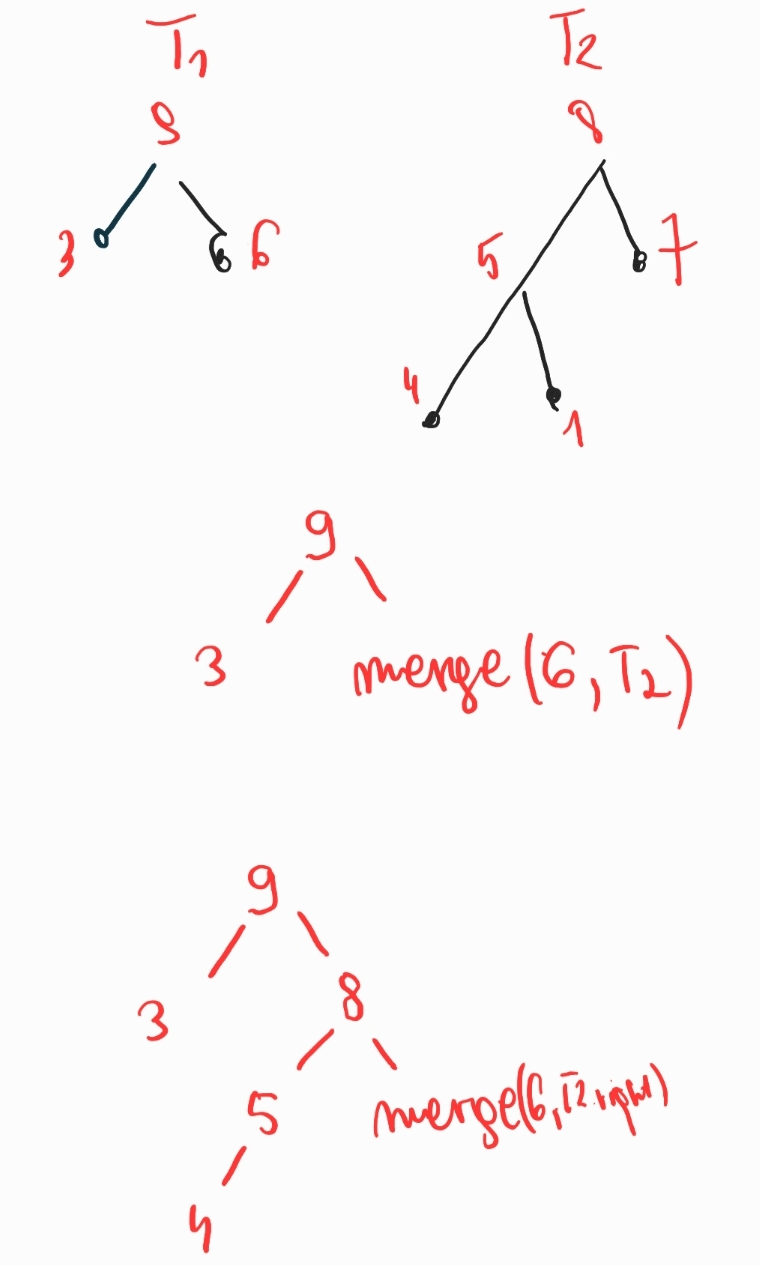
\includegraphics[scale=0.5]{zad5_1.png}
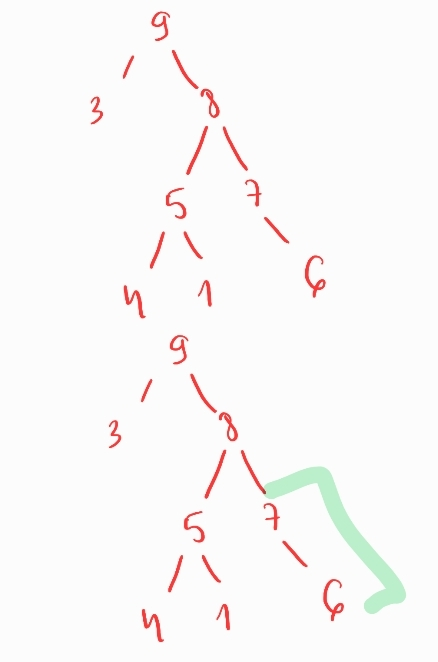
\includegraphics[scale=0.5]{zad5_2.png}
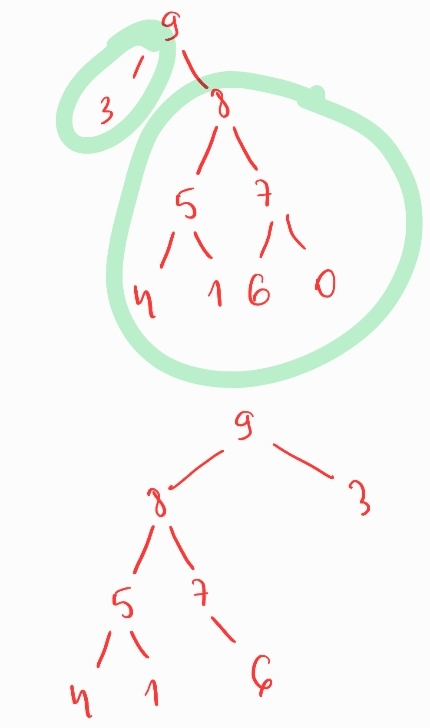
\includegraphics[scale=0.5]{zad5_3.png}

\section{Zadanie 6}

Drzewo BST to drzewo, które ma strukturę drzewa binarnego. Każdy węzeł posiada atrybut key, left, right, father. Klucze w tym drzewie sa przechowywane w taki sposób, aby jeśli y jest węzłem znajdującym się w lewy poddrzewie węzła x, to y.key $\leq$ x.key. Jeśli y jest węzłem znajudjącym się w prawym poddrzewie węzła x, to y.key $\geq$ x.key.
Na drzewach przeszukiwań binarnych możemy przeprowadzić wiele operacji. Insert, Delete, Search, Max, Min, Transplant
Możemy również przeprowadzić operacje rotacji w lewo i w prawo. Są to operacje odwrotne.

ROTACJA W PRAWO
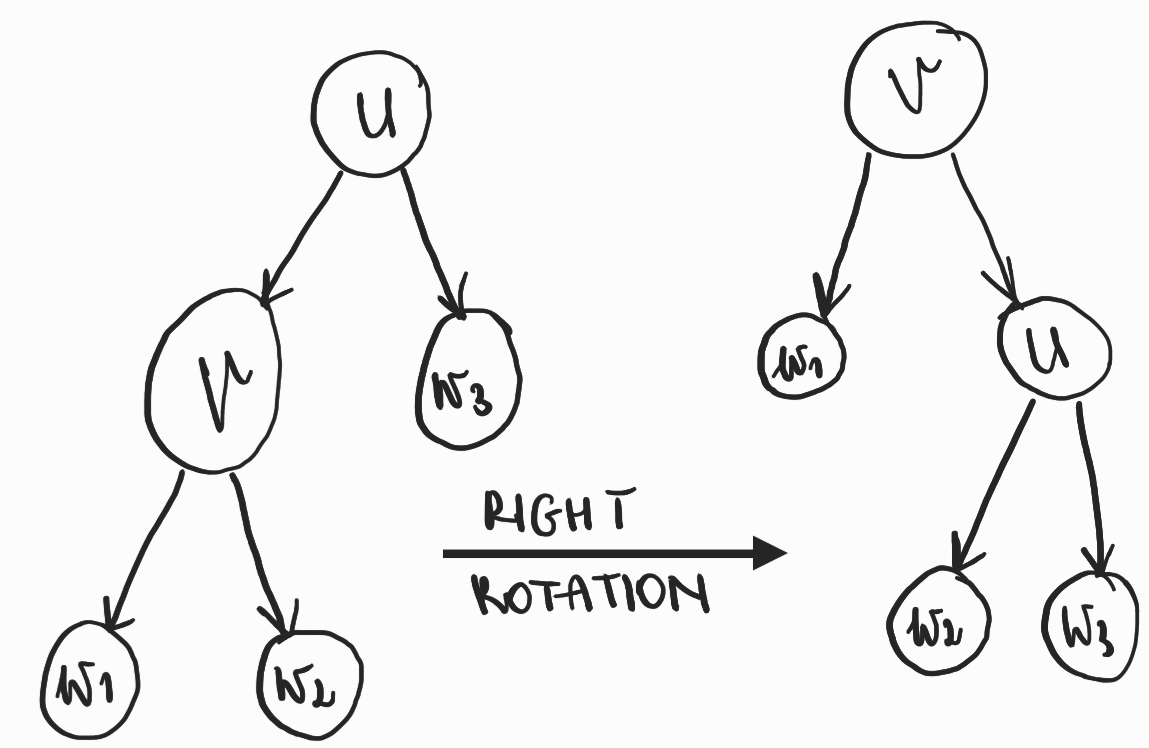
\includegraphics[scale=0.2]{zad6_1.png}
ROTACJA W LEWO to odwrotna operacja do rotacji w prawo
Rozpiszmy jak wygląda rotacja w lewo
\begin{lstlisting}
def left_rotate(T, v):
    u = v.right
    v.right = u.left
    
    if u.left != null:
        u.left.father = v
    u.father = v.father
    
    if v.father == null:
        T.root = u
    else if v == v.father.left:
        v.father.left = u
    else:
        v.father.right = u
        
    u.left = v
    v.father = u
\end{lstlisting}
wierzchołek v to wierzchołek, który chcemy zrotować z wierzchołkiem, który jest jego prawym synem. Oznaczać go będziemy jako u.

Pokażemy, że dowolne drzewo BST da się przekształcić w inne dowolne drzewo BST (,które jest z budowane z tych samych kluczy).
Wystarczy pokazać, że wiedząć jaki jest korzeń drzewa w drzewie docelowym jesteśmy wstanie "wywindowaś" rotacjami odpowiedni wierzchołek do korzenia w drzewie startowym, a następnie zrobić to samo na jego pod drzewach.

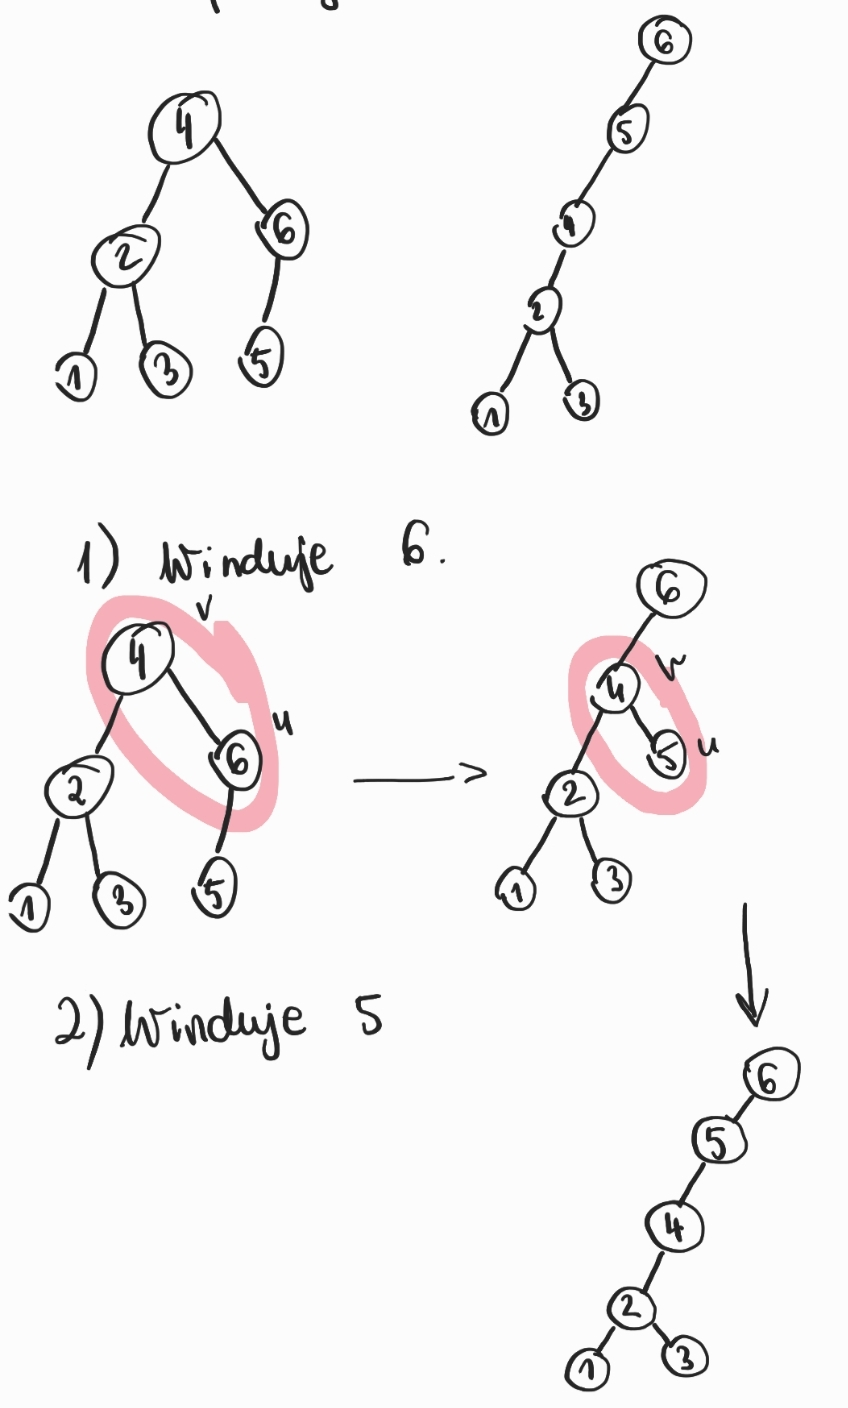
\includegraphics[scale=0.2]{zad6_2.png}

Rozwiązanie to działa ponieważ za każdym razem gdy rotujemy wierzchołek, który chcemy aby był korzeniem, z jego rodzicem to zwiększamy poziom jego położenia, a co za tym idzie kiedyś dotrzemy do korzenia.

Zatem plan działania jet taki:
1) Patrzymy na drzewo docelowe i patrzymy jaki jest oczekiwany korzeń.
2) Znajudjemy wartość tego korzenia w drzewie startowym.
3) Używamy algorytmu do podciągnięcia wierzchołka do korzenia.

Wiemy, że po wykonaniu jednego takiego ciągu operacji oba drzewa (startowe i docelowe) mają w prawym i lewym poddrzewie odpowiednio takie same wartości. WYnika to z własności drzew BST.
Jedyny co może się między  nimi różnić to kształt tych poddrzew. 
W takim razie należy kontunować wywołanie tych 3 kroków na dwóch poddrzewach drzewa startowego

Złożoność czasowa: O(n*logn)

\section{Zadanie 7}

IDEA:
Będziemy schodzić po drzewie od korzenia w dół i w każdym takim kroku odpowiednio rozdzielimy je na dwa poddrzewa. Jedno o elementach mniejszych niż klucz i drugie większe badź równe kluczowi.
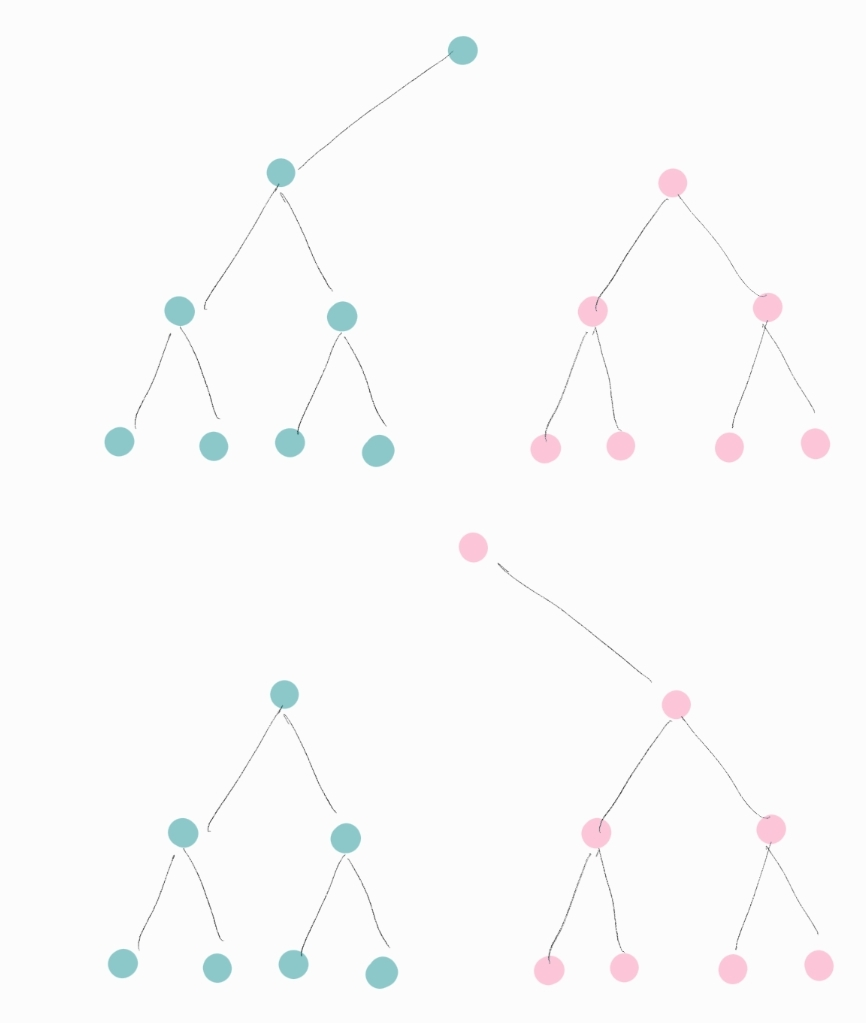
\includegraphics[scale=0.5]{7_1.png}

Przykład;
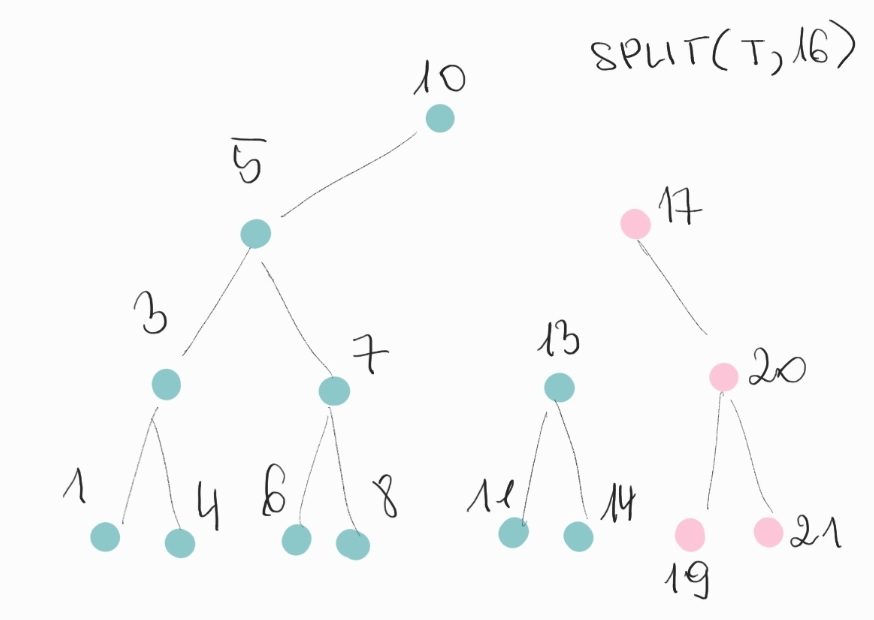
\includegraphics[scale=0.5]{7_2.png}
Procedura podziału zajmie nam $O(lg n)$, ponieważ wysokość drzewa jet logarytmiczna.

Stworzymy operacje Join(T1, x, T2), która jako argumenty przyjmuje dwa drzewa, które są drzewami AVL.
Element x jest większy od wszystkich elelemtnów w drzewie T1 i mniejszy od wszystkich elementów w drzewie T2.
Mamy dwa przypadki:
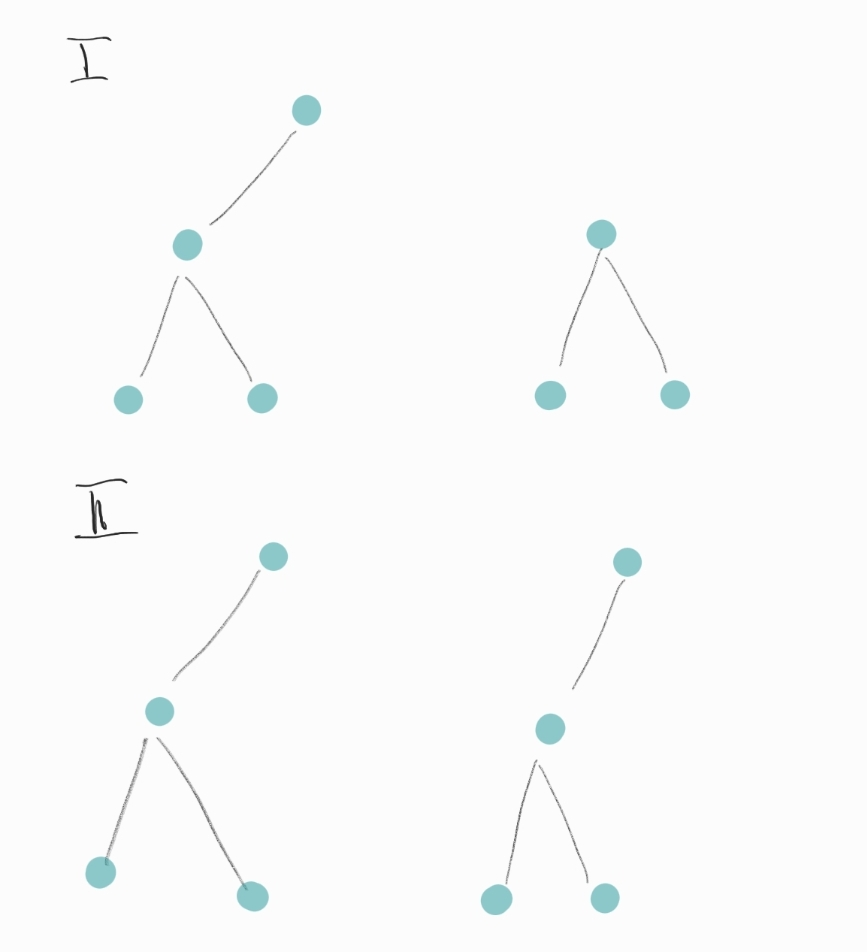
\includegraphics[scale=0.5]{7_3.png}
1) Joinujemy dwa drzew z czego jedno jest avl drugie ma "wystającego" rodzica. Wtedy "wystającego" rodzica odcinamy, drzewo staje sie drzewem AVL a odciety korzeń zapisujemy pod x.
2) Joinujemy dwa drzewa, które nie są AVL, z jedynm z nich postępujemy tak samo jak w przypadku 1, a w drugim odcinamy korzeń i po operacji join wykonujemy operacje insert na drzewie AVL.



Łącząc dwa drzewa AVL nie mamy pewności czy całe drzewo będzie AVL. Wiemy za to, że zaborzenie takiego drzewa będzie na poziomie korzenia. Zatem musimy wykonać odpowiednią ilość rotacji.
Jeśli balans jest dodatni, czyli lewe drzewo zaburza to wykonujemy prawą rotację, wpp. wykonujmey lewą rotację.

Joinować będziemy dwa drzewa o najmniejszej wysokości, tak aby wykonać jak najmniej rotacji. Oznaczmy wysokości drzew od najmniejszego do największego - $h_1, h_2, h_3, ..., h_m$ i wiemy, że $m\leq log_2 n$

Policzmy ile roatacji wykonujemy:

$h_2 - h_1 + h_3 - h_2' + h_4 - h_3' + \ldots + h_m - h_{m-1} \leq h_m - h_1 \le h_m$\\
$-h_1 + (h_2 - h_2) + (h_3 - h_3) + \ldots +(h_{m-1} -h_{m-1}) + h_m = h_m - h_1 \le h_m\\ \le \log_2n $

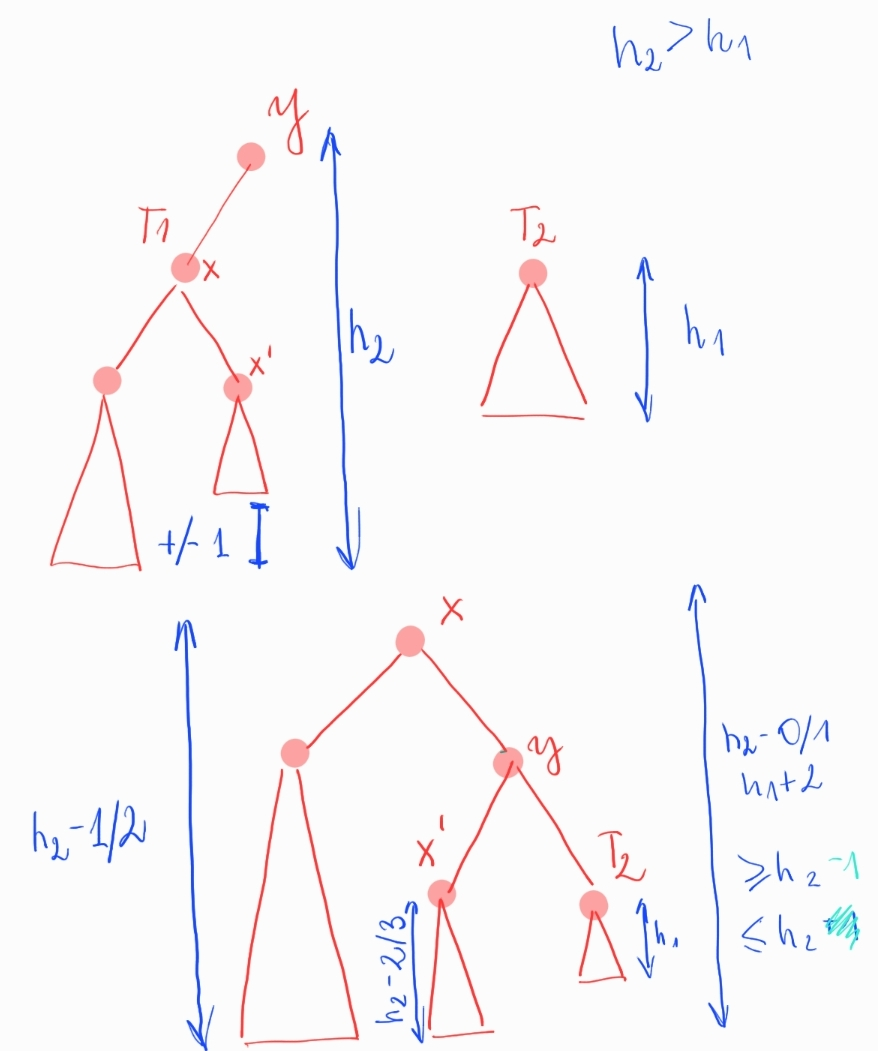
\includegraphics[scale=0.5]{7_4.png}

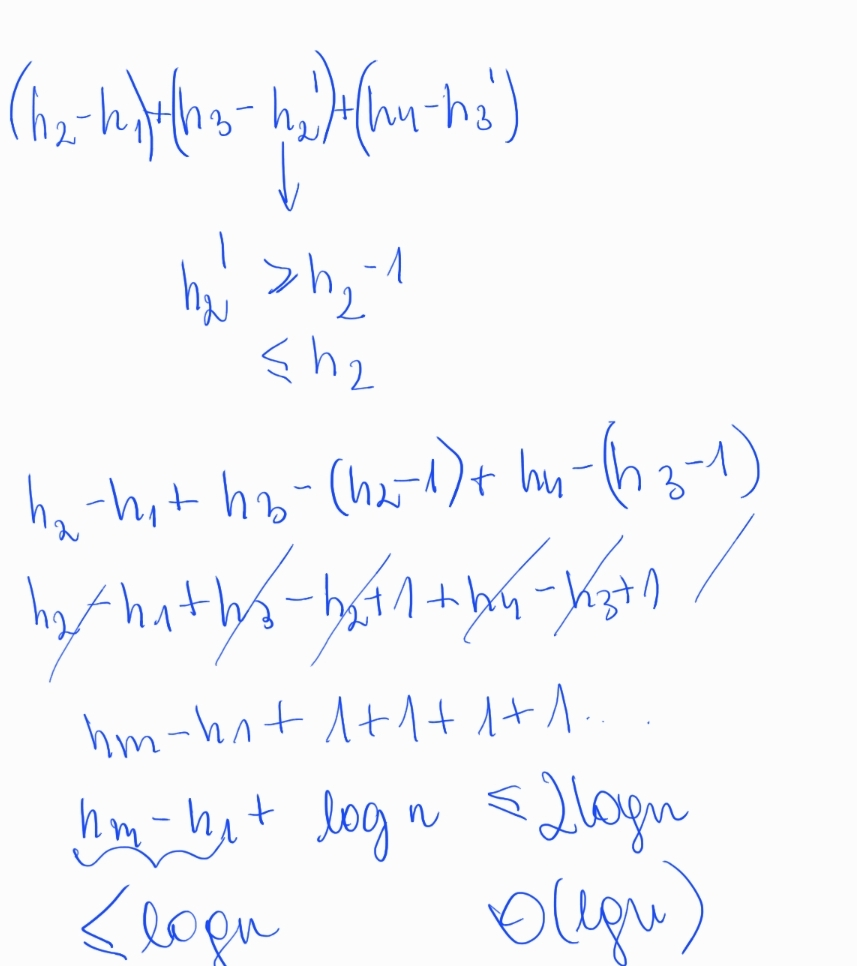
\includegraphics[scale=0.5]{7_5.png}


\section{Zadanie 8}


Proponowana struktura: drzewa czerwono-czarne
Drzewo czerwono czarne to drzewo BST o włsnościach:
- Każdy węzeł jest albo czerwony albo czarny
- Korzeń jest czarny
- Gdy węzeł jest czerwony, to obaj jego synowie są czarni
- Każda ścieżka z ustalonego węzła do liścia ma tyle samo czarnych węzłów

Dodatkowo będziemy pamiętać wartość minDiff - przy dodawaniu nowego wierzchołka musimy znaleźć pierwszy element większy od niego i pierwszy element mniejszy od niego i wziąć mniejszą z różnic.

OPERACJA INSERT 
\begin{lstlisting}
    def insert(T, z):
        minDiff = min(minDiff, ceiling(z) - z)
        minDiff = min(minDiff, z - floor(z)) 
        y = T.nil
        x = T.root
        #rozpoczynamy przeglad w korzeniu i przeciagamy na dol odpowiednio  w lewo 
        #lub w prawo az napotkamy wartosc nil; tam wstawimy nasz element
        while x != T.nil: 
            y = x
            if z.key < x.key:
                x = x.left
            else x = x.right
        z.father = y
        #jesli okaze sie ze element nie ma ojca to jest to korzen
        if y == T.nil:
            T.root = z
        #ustawiamy odpowienio elemetn na lewo lub prawe dziecko
        elif z.key < y.key:
            y.left = z
        else y.right = z
        z.left = T.nil
        z.right = T.nil
        z.color = 'RED'
        insert_fix(T, z)
\end{lstlisting}
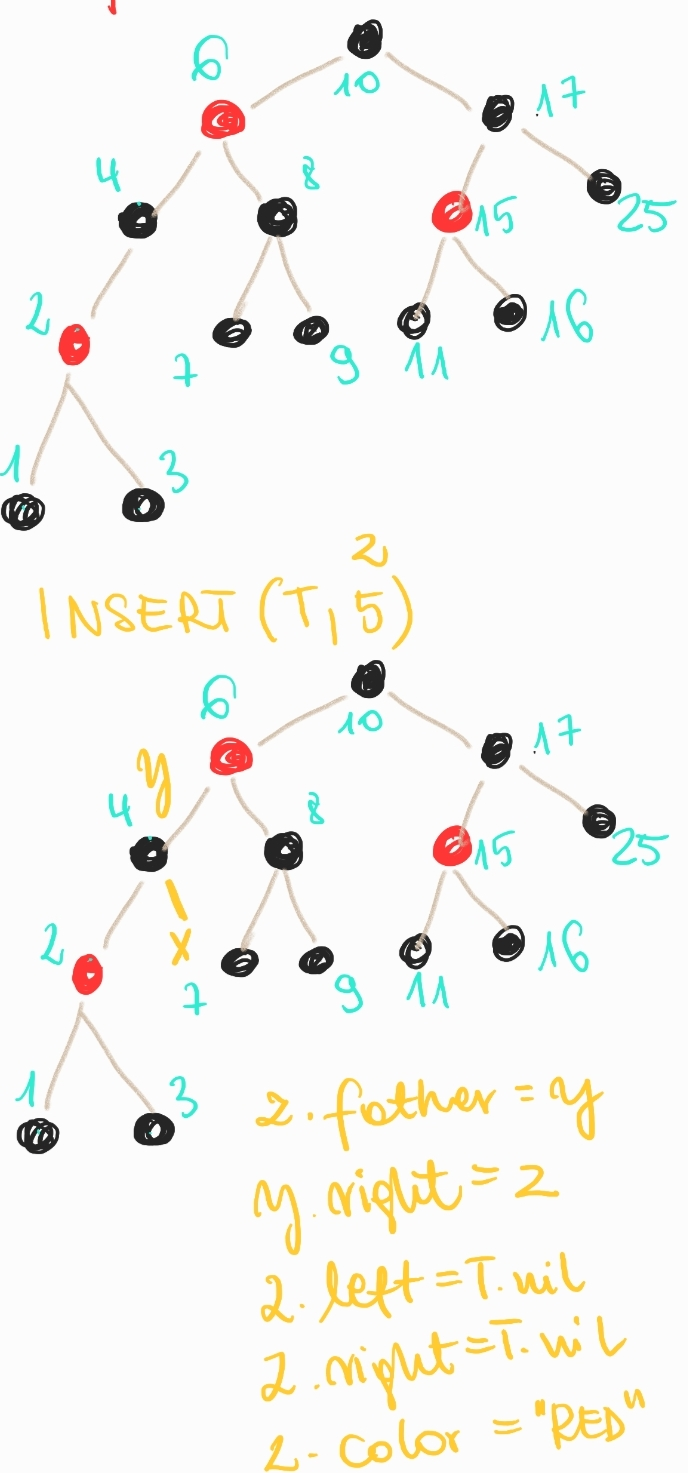
\includegraphics[scale=0.5]{zad8_1.png}
Mamy 3 przypadki, które niszczą nam struktuę drzewa czerwono-czarnego:
1) brat ojca wstawionego elemetnu jest czerwony
2) brat ojca wstawionego elemetnu jest czarny i wstawiony element jest prawym synem
3) brat ojca wstawionego elemetnu jest czarny i wstawiony element jest lewym synem
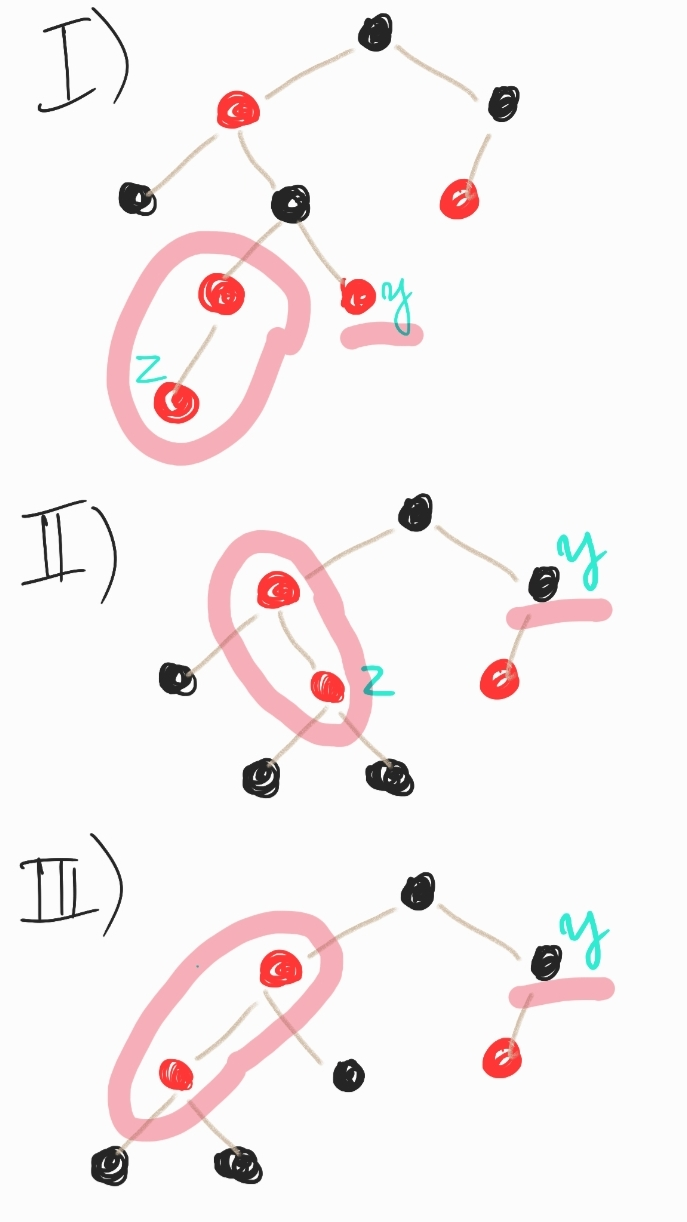
\includegraphics[scale=0.5]{zad8_2.png}

\begin{lstlisting}
def insert_fix(T, z):
    if z.father == z.father.father.left:
        y = z.father.father.rigth
        if y.color == 'RED':
            z.father.color = 'BLACK'
            y.color = 'BLACK'
            z.father.father.color = 'RED'
            z = z.father.father
        else 
            if z == z.father.right:
                z = z.father
                left_rotate(T,z)
            z.father.color = 'BLACK'
            z.father.father.color = 'RED'
            right_rotate(T, z.father.father)
    else
        y = z.father.father.left
        if y.color == 'RED':
            z.father.color = 'BLACK'
            y.color = 'BLACK'
            z.father.father.color = 'RED'
            z = z.father.father
        else 
            if z == z.father.left:
                z = z.father
                left_rotate(T,z)
            z.father.color = 'BLACK'
            z.father.father.color = 'RED'
            right_rotate(T, z.father.father)
    T.root.color = 'BLACK'
\end{lstlisting}

OPERACJA DELETE
operacja transplant służy do przesuwania poddrzew w  drzewie wyszukiwań binarnych. Wstawiw jedno poddrzewo w miejsce drugiego w jego ojcu. Ojciec u staje się ojcem v, a v zostaje synem ojca u.
\begin{lstlisting}
def transplant(t, u, v):
    if u.father == T.nil:
        T.root = v
    elif u == u.father.left:
        u.father.left = v
    else u.father.right = v
    v.father = u.father

def delete(T, z):
    y = z
    y-original-color = y.color
    #gdy lewo poddrzewo jest puste
    if z.left == T.nil
        x = z.right
        transplant(T, z, z.right)
    #gdy prawe poddrzewo jest puste
    elif z.right == T.nil
        x = z.left
        transplant(T, z, z.left)
    else 
        y = minimum(z.right)
        y-orginal-color = y.color
        x = y.right
        if y.father == z:
            x.father = y
        else 
            transplant(T, y, y.right)
            y.right = z.right
            y.right.father = y
        tranplant(T, z, y)
        y.left = z.left
        y.left.father = y
        y.color = z.color
    if y-orginal-color == 'BLACK'
        delete-fix(T, x)

def delete-fix(T, x):
    while x != T.root and x.color == 'BLACK':
        if x == x.father.left:
            w = x.father.right
            if w.color == 'RED':
                w.color = 'BLACK'
                x.father.color = 'RED'
                left_rotate(T, x.father)
                w = x.father.right
            if w.left.color == 'BLACK' and w.right.color = 'BLACK':
                w.color = 'RED'
                x = x.father
            else
                if w.right.color == 'BLACK':
                    w.left.color = 'BLACK'
                    w.color = 'RED'
                    right_rotate(T, w)
                    w = x.father.right
                w.color = x.father.color
                x.father.color = 'BLACK'
                w.right.color = 'BLACK'
                left_rotate(T, x.father)
                x = T.root
        else
            w = x.father.left
            if w.color == 'RED':
                w.color = 'BLACK'
                x.father.color = 'RED'
                left_rotate(T, x.father)
                w = x.father.left
            if w.right.color == 'BLACK' and w.left.color = 'BLACK':
                w.color = 'RED'
                x = x.father
            else
                if w.left.color == 'BLACK':
                    w.right.color = 'BLACK'
                    w.color = 'RED'
                    right_rotate(T, w)
                    w = x.father.left
                w.color = x.father.color
                x.father.color = 'BLACK'
                w.left.color = 'BLACK'
                left_rotate(T, x.father)
                x = T.root
    x.color = 'BLACK'
        
\end{lstlisting}
OPERACJA FLOOR I CEILING
\begin{lstlisting}

def ceiling(T, z):
    if T == none:
        return none 
    if T.value == z:
        return z 
    if T.value < z:
        return ceiling(T.right, z)
    left_celing = ceiling(T.left, z)
    if left_ceiling is not none:
        return left_ceiling
    else:
        return T.value 


def floor(T, z):
    if T == none:
        return none 
    if T.value == z:
        return z 
    if T.value > z:
        return floor(T.left, z)
    right_floor = floor(T.right, z)
    if right_floor is not none:
        return right_floor
    else:
        return T.value 
\end{lstlisting}


\section{Zadanie 9}
Chcielibyśmy trzymać w indeksach wskaźniki. Trzymamy dwa drzewa - jedno z elementami na miejscach parzytych, drugie z elementami na miejscach nieparzystych. Gdy dodajemy nowy element to sprawdzamy ile jest elementów w drzewie i dodajemy do drzewa z odpowiednia parzystoscia. 

Jesli usuwamy jakis element na pozycji i, to wszystkie elementy na pozycjach kolejnych zmieniaja parzystosc. 
Czyli to co musimy zrobic to przepiac elementy z drzewa nieparzystego do drzewa parzystego i odwrotnie.

Czyli nasz insert jest w czasie $O(\log n)$, a delete w czasie $O(2\log n)$, czyli $O(\log n)$.
Jak z findem - również jest w czasie $O(\log n)$, wystarczy wejść do odpowiedniego drzewa i znaleźć podany indeks jak w BST i zwrócić wartość trzymaną w danym wierzchołku.

Okej, a co z sumą elementów na miejscach parzystych. Jest to po prostu suma elementów z drzewa parzystego. No ale nie chcielibyśmy robić tak, że idziemy po wszystkich elementach i trzymamy sumę. Idea jest taka, że w wierzchołku trzymamy sumę wszystkich elementów w poddrzewie. 
Wtedy będzie tak, że jak przepniemy elementy z drzewa nieparzystego do drzewa parzystego to musimy zaktualizować sumy w wierzchołkach na ścieżce od korzenia do wierzchołka który dodaliśmy. 

Żeby to wszystko zachodziło musimy mieć drzewo dość zbalansowane.


Zachodzi tu jeszcze jeden problem - nie będziemy pamiętać dobrze wskaźników - bo jeśli usuniemy jakiś element i wszystkie następne elementy zmniejszą swój wskaźnik o 1, to nie będzie przecież tego robić ręcznie, więc chcemy się pozbyć idei miejsca w tabeli. No ale jeśli wiemy jakie elementy z poddrzewa będą przepięte, to możemy dodać w korzeniu informacje o tym o ile jest zmieniony wskaźnik (wartość którą trzeba dodać do wskaźników aby mieć obecnie dobry wskaźnik).



Użyjemy drzew splay. W drzewach splay jak chcemy splitować drzewa, to robimy tak, że ustawiamy element przed splitem na splay i odcinamy prawe drzewo. W takim razie gdy mamy delete to robimy splay na id mniejszym o 1 niż chcemy usunąć i wtedy mamy po prawej wszystkie elementy większe niż w danym wskaźniku i możemy je odciąć. 
Teraz dochodzi taki szczegół - gdy będziemy robić jakąś rotację, to może być tak, że zgubimy poprawne wartościowanie id. No ale jeśli tak będzie, to musimy zawsze znaleźć jakiś wierzchołek który będziemy odcinać. Czyli jeśli w jakimś wierzchołku było np. że id mamy zwiększyć o 3 oraz jakiś wierzchołek w poddrzewie będziemy usuwać z tego poddrzewa i przepinać go gdzieś indziej, to do tego wierzchołka musimy dojść. Czyli idąc w dół możemy aktualizować wartość wskaźnika.
Czyli załóżmy, że idziemy np. ojciec -> lewy syn -> prawy syn i ojciec ma wartość do zwiększenia równą 3.
Wtedy zrobimy tak, że do id ojca dodamy 3, wartość do zwiększenia ustawimy na 0, do lewego i prawego syna dodamy wartość do zwiększenia równą wartości ojca i zrobimy rekurencje na to gdzie chcemy iść, czyli lewy syn.



\section{Zadanie 10}


Dla każdego wierzchołka pamiętamy czy sąsiad jest większy
0 - nie jest większy
1 - większy 

jeśli 2x mamy 0 to jest równe 
jeśli mamy w jednym 1 a w drugim 0 to wiemy który większy

\egroup
\end{document}